\documentclass[11pt]{article}

% some definitions for the title page
\newcommand{\reporttitle}{Aim of the Project}
\newcommand{\reportdescription}{}

% load some definitions and default packages
%%%%%%%%%%%%%%%%%%%%%%%%%%%%%%%%%%%%%%%%%
% University Assignment Title Page 
% LaTeX Template
% Version 1.0 (27/12/12)
%
% This template has been downloaded from:
% http://www.LaTeXTemplates.com
%
% Original author:
% WikiBooks (http://en.wikibooks.org/wiki/LaTeX/Title_Creation)
%
% License:
% CC BY-NC-SA 3.0 (http://creativecommons.org/licenses/by-nc-sa/3.0/)
% 
%
%%%%%%%%%%%%%%%%%%%%%%%%%%%%%%%%%%%%%%%%%
%----------------------------------------------------------------------------------------
%	PACKAGES AND OTHER DOCUMENT CONFIGURATIONS
%----------------------------------------------------------------------------------------
\usepackage[a4paper,hmargin=2.0cm,vmargin=1.0cm,includeheadfoot]{geometry}
\usepackage{textpos}

\usepackage[square,numbers]{natbib} % for bibliography
\usepackage[nottoc]{tocbibind} % Includes "References" in the table of contents
\bibliographystyle{unsrtnat}

\usepackage{tabularx,longtable,multirow,subfigure,caption}%hangcaption
\usepackage{fancyhdr} % page layout
\usepackage{url} % URLs
\usepackage[english]{babel}
\usepackage{amsmath}
\usepackage{graphicx}
\usepackage{scalerel}
\usepackage{dsfont}
\usepackage{epstopdf} % automatically replace .eps with .pdf in graphics
\usepackage{backref} % needed for citations
\usepackage{array}
\usepackage{latexsym}

\usepackage[pdftex,pagebackref,hypertexnames=false,colorlinks]{hyperref} % provide links in pdf
\usepackage{booktabs}
\usepackage{wrapfig}
\usepackage{caption}  % Required for \captionof
\usepackage{float} % for H option in figures
\usepackage{amssymb}
\usepackage{amsmath}
\usepackage{csquotes}
% \usepackage{subcaption} % causes a compilation error after changing back to natbib referencing... 

\hypersetup{pdftitle={},
  pdfsubject={}, 
  pdfauthor={},
  pdfkeywords={}, 
  pdfstartview=FitH,
  pdfpagemode={UseOutlines},% None, FullScreen, UseOutlines
  bookmarksnumbered=true, bookmarksopen=true, colorlinks,
    citecolor=black,%
    filecolor=black,%
    linkcolor=black,%
    urlcolor=black}

\usepackage[all]{hypcap}

%%%%%%%%%%%%%%%%%%%%%%%%%%%%%%%%%%%%%%%%%%%%%%%%%%%%%%%%%%%%%%%%%%%%%%%%%%%%%%%%
% LISTINGS ammendments
%%%%%%%%%%%%%%%%%%%%%%%%%%%%%%%%%%%%%%%%%%%%%%%%%%%%%%%%%%%%%%%%%%%%%%%%%%%%%%%%
\usepackage{listings}

\lstset
{ %Formatting for code in appendix
    language=Matlab,
    basicstyle=\footnotesize,
    % numbers=left,
    stepnumber=1,
    showstringspaces=false,
    tabsize=1,
    breaklines=true,
    breakatwhitespace=false,
    frame=single,
    columns=fullflexible,
    postbreak=\mbox{\textcolor{red}{$\hookrightarrow$}\space},
}

%\usepackage{color}
%\usepackage[tight,ugly]{units}
%\usepackage{float}
%\usepackage{tcolorbox}
%\usepackage[colorinlistoftodos]{todonotes}
% \usepackage{ntheorem}
% \theoremstyle{break}
% \newtheorem{lemma}{Lemma}
% \newtheorem{theorem}{Theorem}
% \newtheorem{remark}{Remark}
% \newtheorem{definition}{Definition}
% \newtheorem{proof}{Proof}


%%% Default fonts
\renewcommand*{\rmdefault}{bch}
\renewcommand*{\ttdefault}{cmtt}


%%% Default settings (page layout)
\setlength{\parindent}{0em}  % indentation of paragraph
\setlength{\parskip}{.3em}

% \setlength{\parindent}{0em}  % indentation of paragraph

\setlength{\headheight}{14.5pt}
\pagestyle{fancy}
\renewcommand{\chaptermark}[1]{\markboth{\chaptername\ \thechapter.\ #1}{}}
%\fancyhead[RO]{\sffamily \textbf{\thepage}} %Page no.in the right on even pages
%\fancyhead[LE]{\sffamily \textbf{\thepage}} %Page no. in the left on odd pages

\fancyfoot[ER,OL]{\thepage}%Page no. in the left on
%odd pages and on right on even pages
\fancyfoot[OC,EC]{\sffamily }
\renewcommand{\headrulewidth}{0.1pt}
\renewcommand{\footrulewidth}{0.1pt}
\captionsetup{margin=10pt,font=small,labelfont=bf}


%--- chapter heading

\def\@makechapterhead#1{%
  \vspace*{10\p@}%
  {\parindent \z@ \raggedright \sffamily
    \interlinepenalty\@M
    \Huge\bfseries \thechapter \space\space #1\par\nobreak
    \vskip 30\p@
  }}

%--- chapter heading

\def\@makechapterhead#1{%
  \vspace*{10\p@}%
  {\parindent \z@ \raggedright \sffamily
    %{\Large \MakeUppercase{\@chapapp} \space \thechapter}
    %\\
    %\hrulefill
    %\par\nobreak
    %\vskip 10\p@
    \interlinepenalty\@M
    \Huge\bfseries \thechapter \space\space #1\par\nobreak
    \vskip 30\p@
  }}

%---chapter heading for \chapter*  
\def\@makeschapterhead#1{%
  \vspace*{10\p@}%
  {\parindent \z@ \raggedright
    \sffamily
    \interlinepenalty\@M
    \Huge \bfseries  #1\par\nobreak
    \vskip 30\p@
  }}
\allowdisplaybreaks
% Here, you can define your own macros. Some examples are given below.

\newcommand{\R}[0]{\mathds{R}} % real numbers
\newcommand{\Z}[0]{\mathds{Z}} % integers
\newcommand{\N}[0]{\mathds{N}} % natural numbers
\newcommand{\C}[0]{\mathds{C}} % complex numbers
% \renewcommand{\vec}[1]{{\boldsymbol{{#1}}}} % vector
\newcommand{\mat}[1]{{\boldsymbol{{#1}}}} % matrix

\usepackage{pifont,mdframed}
\newenvironment{warning}
  {\par\begin{mdframed}[linewidth=1pt,linecolor=black]%
    \begin{list}{}{\leftmargin=1cm
                  \labelwidth=\leftmargin}\item[\Large\ding{43}]}
  {\end{list}\end{mdframed}\par}

\definecolor{lightgray}{gray}{0.9}

\begin{document}

% Include the title page
% Last modification: 2015-08-17 (Marc Deisenroth)
\begin{titlepage}

    \newcommand{\HRule}{\rule{\linewidth}{0.5mm}} % Defines a new command for the horizontal lines, change thickness here
    
    %----------------------------------------------------------------------------------------
    %	LOGO SECTION
    %----------------------------------------------------------------------------------------
    
    
\includegraphics[width = 4cm]{../figures/imperial.pdf}\\[0.5cm] 
    
    \center % Center everything on the page
     
    %----------------------------------------------------------------------------------------
    %	HEADING SECTIONS
    %----------------------------------------------------------------------------------------
    
    \textsc{\LARGE \reporttype}\\[1.5cm] 
    \textsc{\Large Department of Computing}\\[0.5cm] 
    \textsc{\large Imperial College of Science, Technology and Medicine}\\[0.5cm] 
    
    %----------------------------------------------------------------------------------------
    %	TITLE SECTION
    %----------------------------------------------------------------------------------------
    
    \HRule \\[0.4cm]
    { \huge \bfseries \reporttitle}\\ % Title of your document
    \HRule \\[1.5cm]
     
    %----------------------------------------------------------------------------------------
    %	AUTHOR SECTION
    %----------------------------------------------------------------------------------------
    
    \begin{minipage}{0.4\textwidth}
    \begin{flushleft} \large
    \emph{Author:}\\
    \reportauthor % Your name
    \end{flushleft}
    \end{minipage}
    ~
    \begin{minipage}{0.4\textwidth}
    \begin{flushright} \large
    \emph{Supervisor:} \\
    \supervisor % Supervisor's Name
    \end{flushright}
    \end{minipage}\\[4cm]
    
    
    
    
    %----------------------------------------------------------------------------------------
    
    
    %----------------------------------------------------------------------------------------
    %	DATE SECTION
    %----------------------------------------------------------------------------------------
    
    {\large \today} % Date, change the \today to a set date if you want to be precise
    
    
    \vfill % Fill the rest of the page with whitespace
    Submitted in partial fulfillment of the requirements for the \degreetype~of Imperial College London
    
    \end{titlepage}
    

\tableofcontents

\clearpage

\section{Aim}

A patient with a cancerous area needs treatment. A way to treat them is to obtain a 3D CT scan and analyze the data to obtain a segmented area across each slice which highlights the area that is cancerous and requires radiation in order to treat the issue.

\begin{quote}
    The clinical target volume is the area where there is likely microscopic cancer and this area needs to receive sufficient radiation doses to achieve cancer cure. As microscopic cancer cannot be seen on CT, the clinical target volume is not an obvious structure that can be drawn around. The CTV is however constructed based on an Oncologist's knowledge of where each particular cancer is likely to spread to. It is drawn based on guidelines, atlases and clinical information. There are currently no internationally agreed guidelines for exactly how the clinical target volume should be drawn for cervix cancer and practice varies. Practice varies based on how the individual components of the CTV are labelled and this in theory could make it difficult for an AI model to learn patterns (or to generate large quantities of similar quality training data)~\cite{AMLART-data}.
\end{quote}

We have 5 structures given to us as the source data, however, the areas that are cancerous are only the CTVn, CTVp and Parametrium. 

See Section~\ref{ref:DescribingTheData} for each area that needs to be treated with radiation.

\section{Describing the data}\label{ref:DescribingTheData}

\subsection{What are the organs in question?}

We have 5 organs that we aim to develop segmentation models for. These are: Anorectum, Bladder, CTVn, CTVp, and Parametrium.

\subsubsection{Anorectum}

\begin{figure}[H]
    \centering

    \subfigure[Sagittal view of the Anorectum]{
        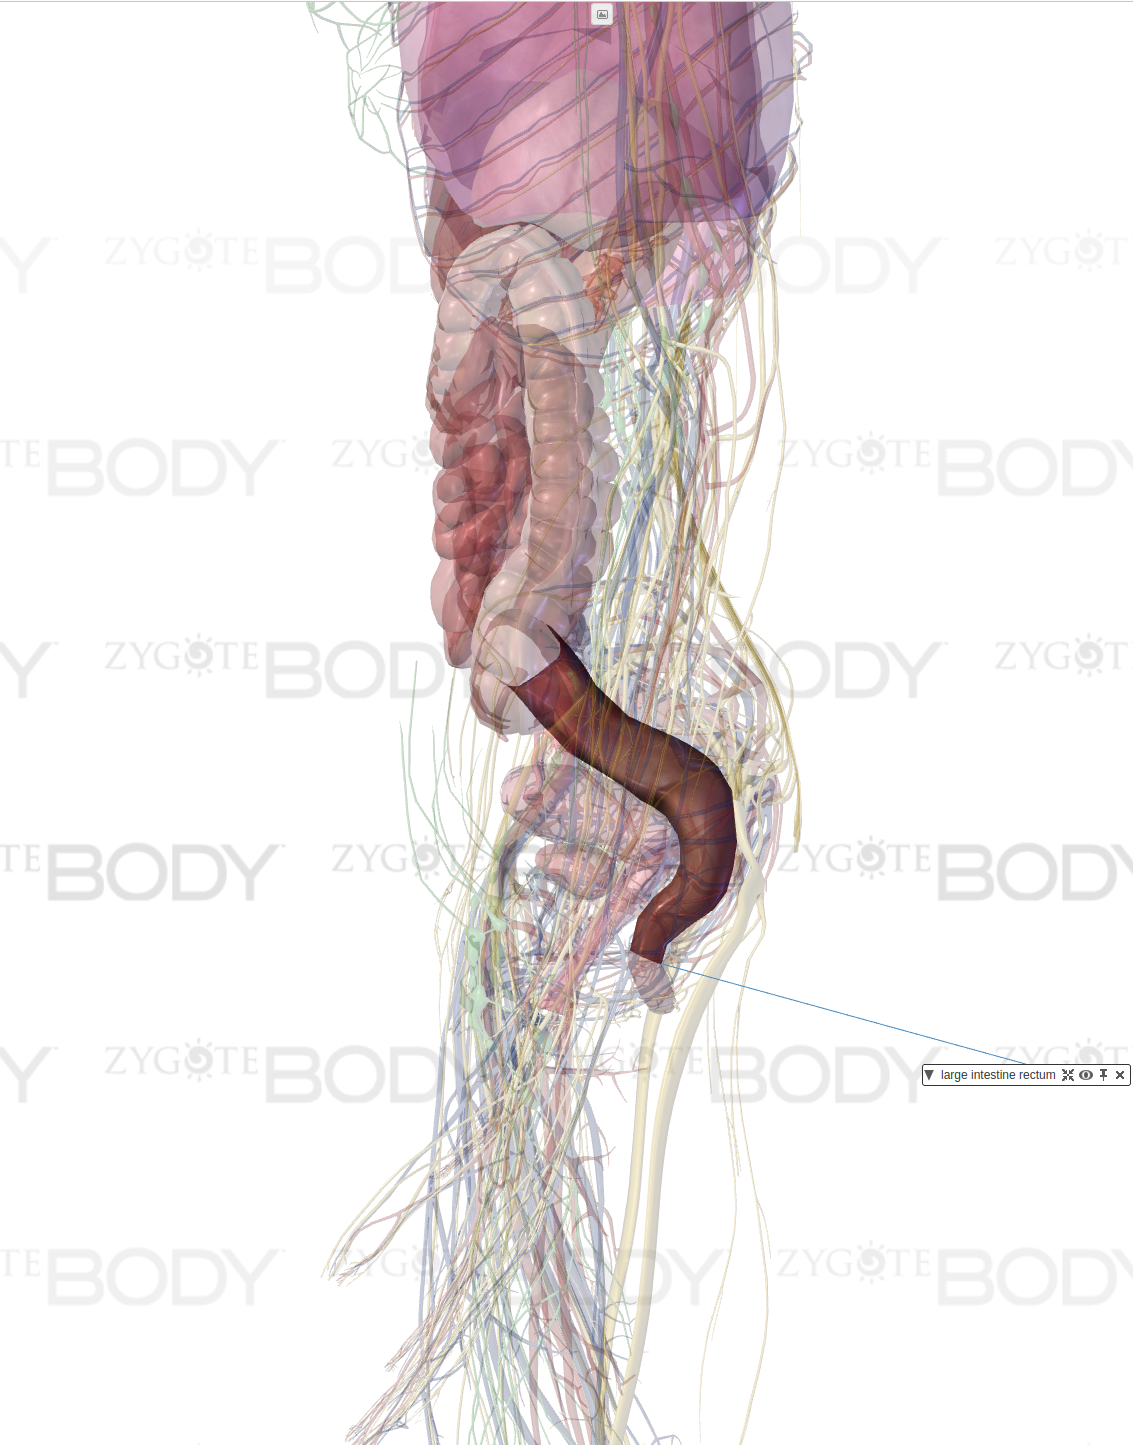
\includegraphics[width=0.3\textwidth]{images/Anorectum-Sagittal.png}\label{fig:anorectumSagittal}
    }
    \subfigure[Coronal view of the Anorectum]{
        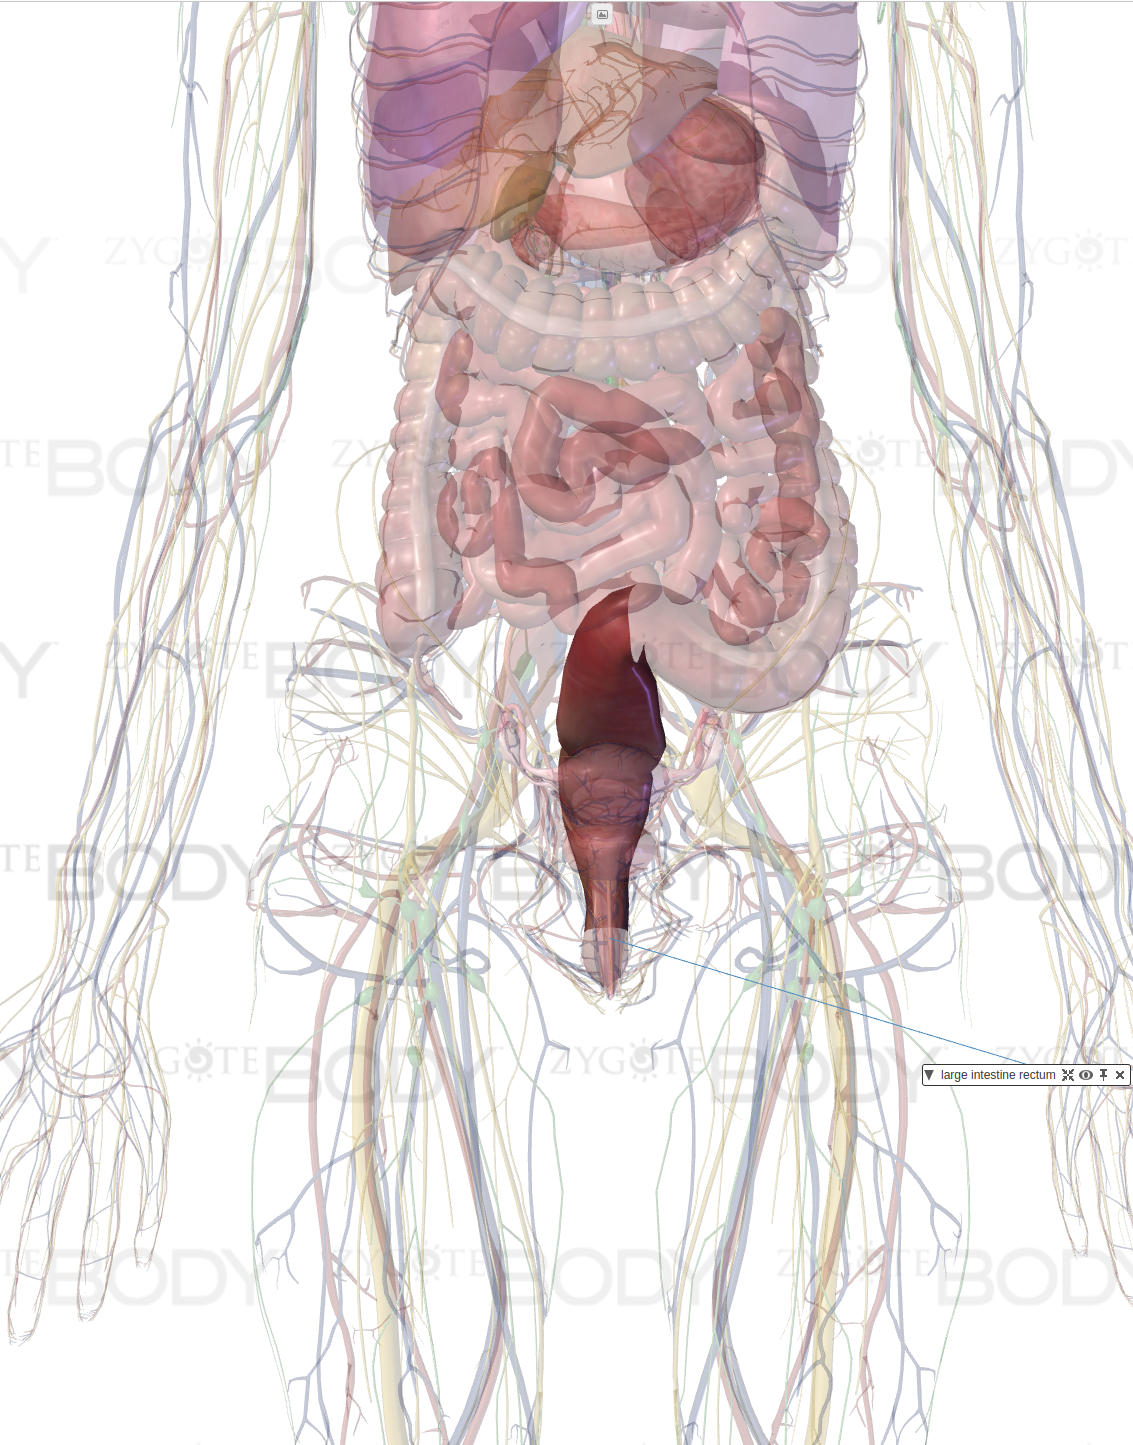
\includegraphics[width=0.3\textwidth]{images/Anorectum-Coronal.png}\label{fig:anorectumCoronal}
    }
    % \subfigure{
    %     \phantom{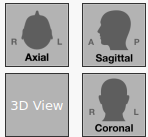
\includegraphics[width=0.4\textwidth]{images/view.png}}
    % }
    % \subfigure[Caption for Figure 3]{
    %     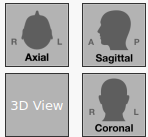
\includegraphics[width=0.4\textwidth]{images/view.png}\label{fig:image3}
    % }
    \caption{Highlighted is the Anorectum}\label{fig:Anorectum}
\end{figure}

\subsubsection{Bladder}

\begin{figure}[H]
    \centering
    \subfigure[Sagittal view of the Bladder]{
        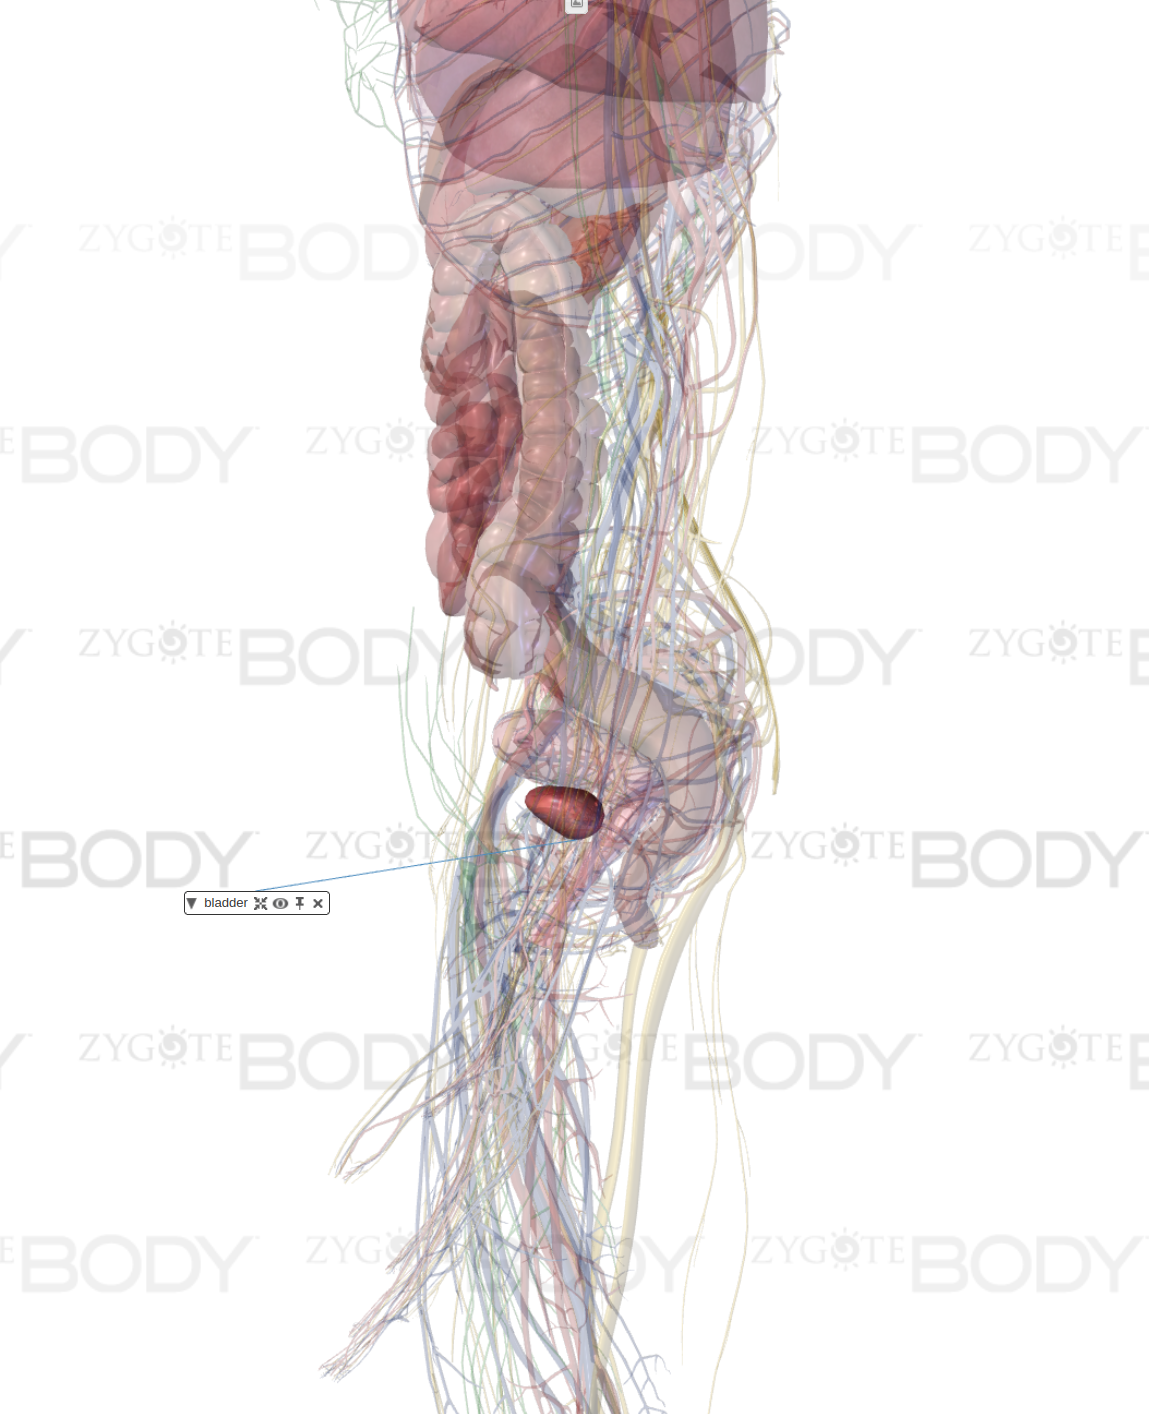
\includegraphics[width=0.3\textwidth]{images/Bladder-Sagittal.png}\label{fig:bladderSagittal}
    }
    \subfigure[Coronal view of the Bladder]{
        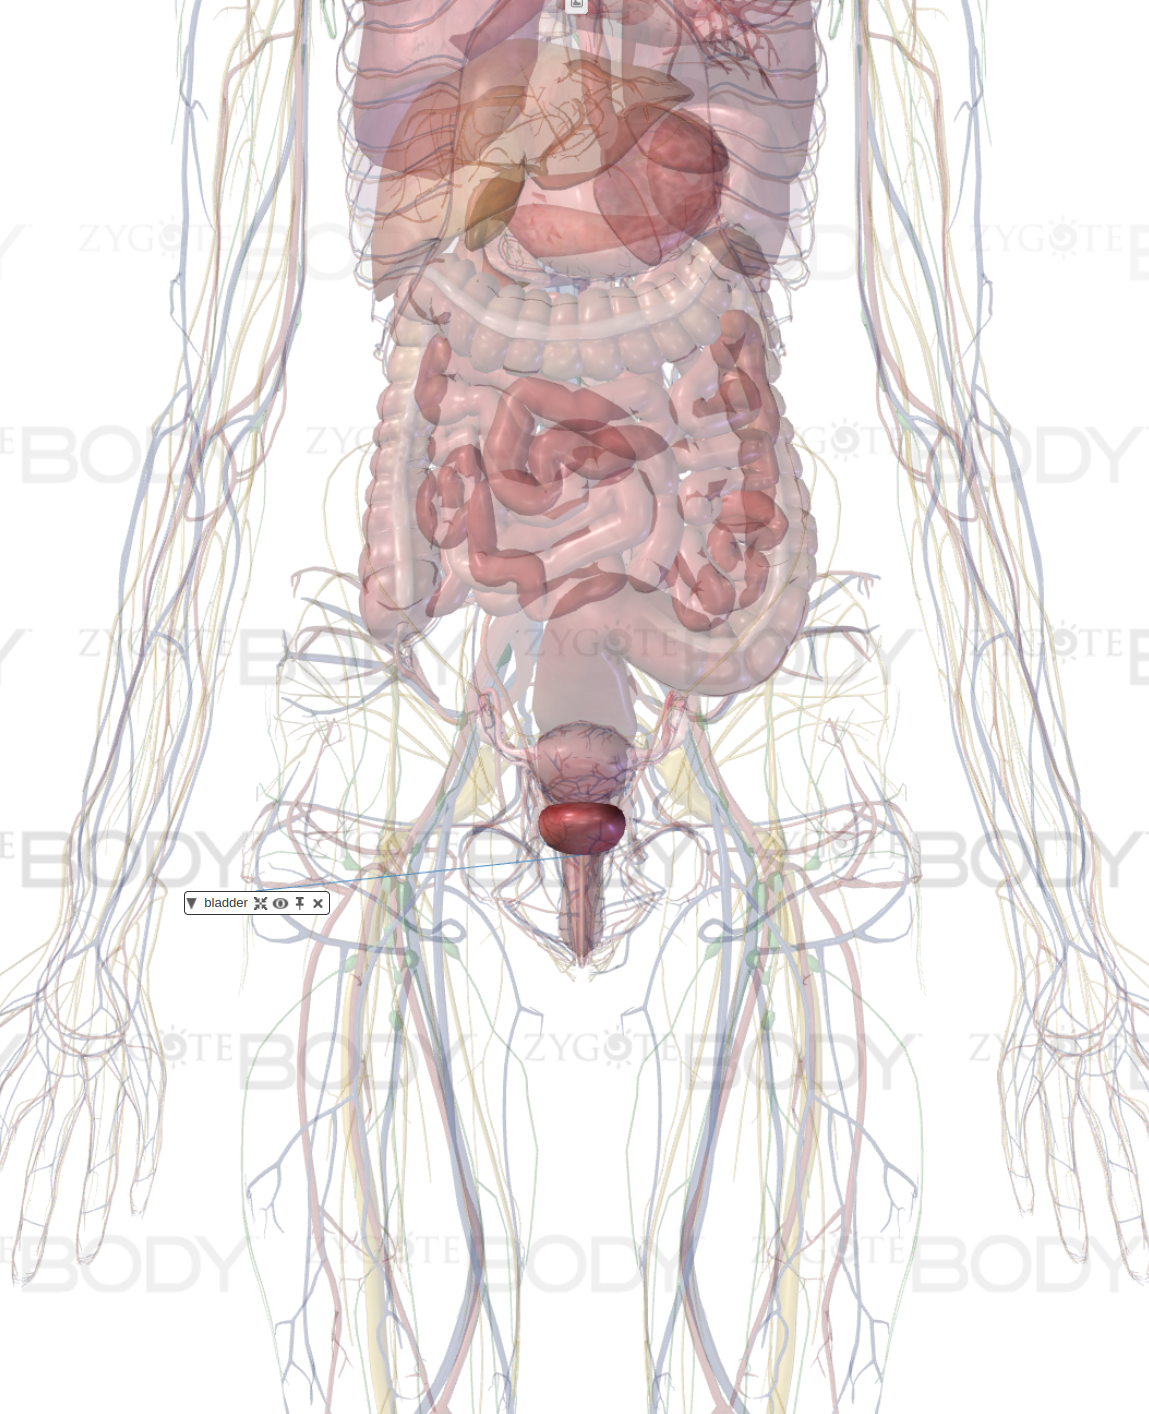
\includegraphics[width=0.3\textwidth]{images/Bladder-Coronal.png}\label{fig:bladderCoronal}
    }
    \caption{Highlighted is the Bladder}\label{fig:Anorectum}
\end{figure}

\subsubsection{CTVp}

\begin{figure}[H]
    \centering
    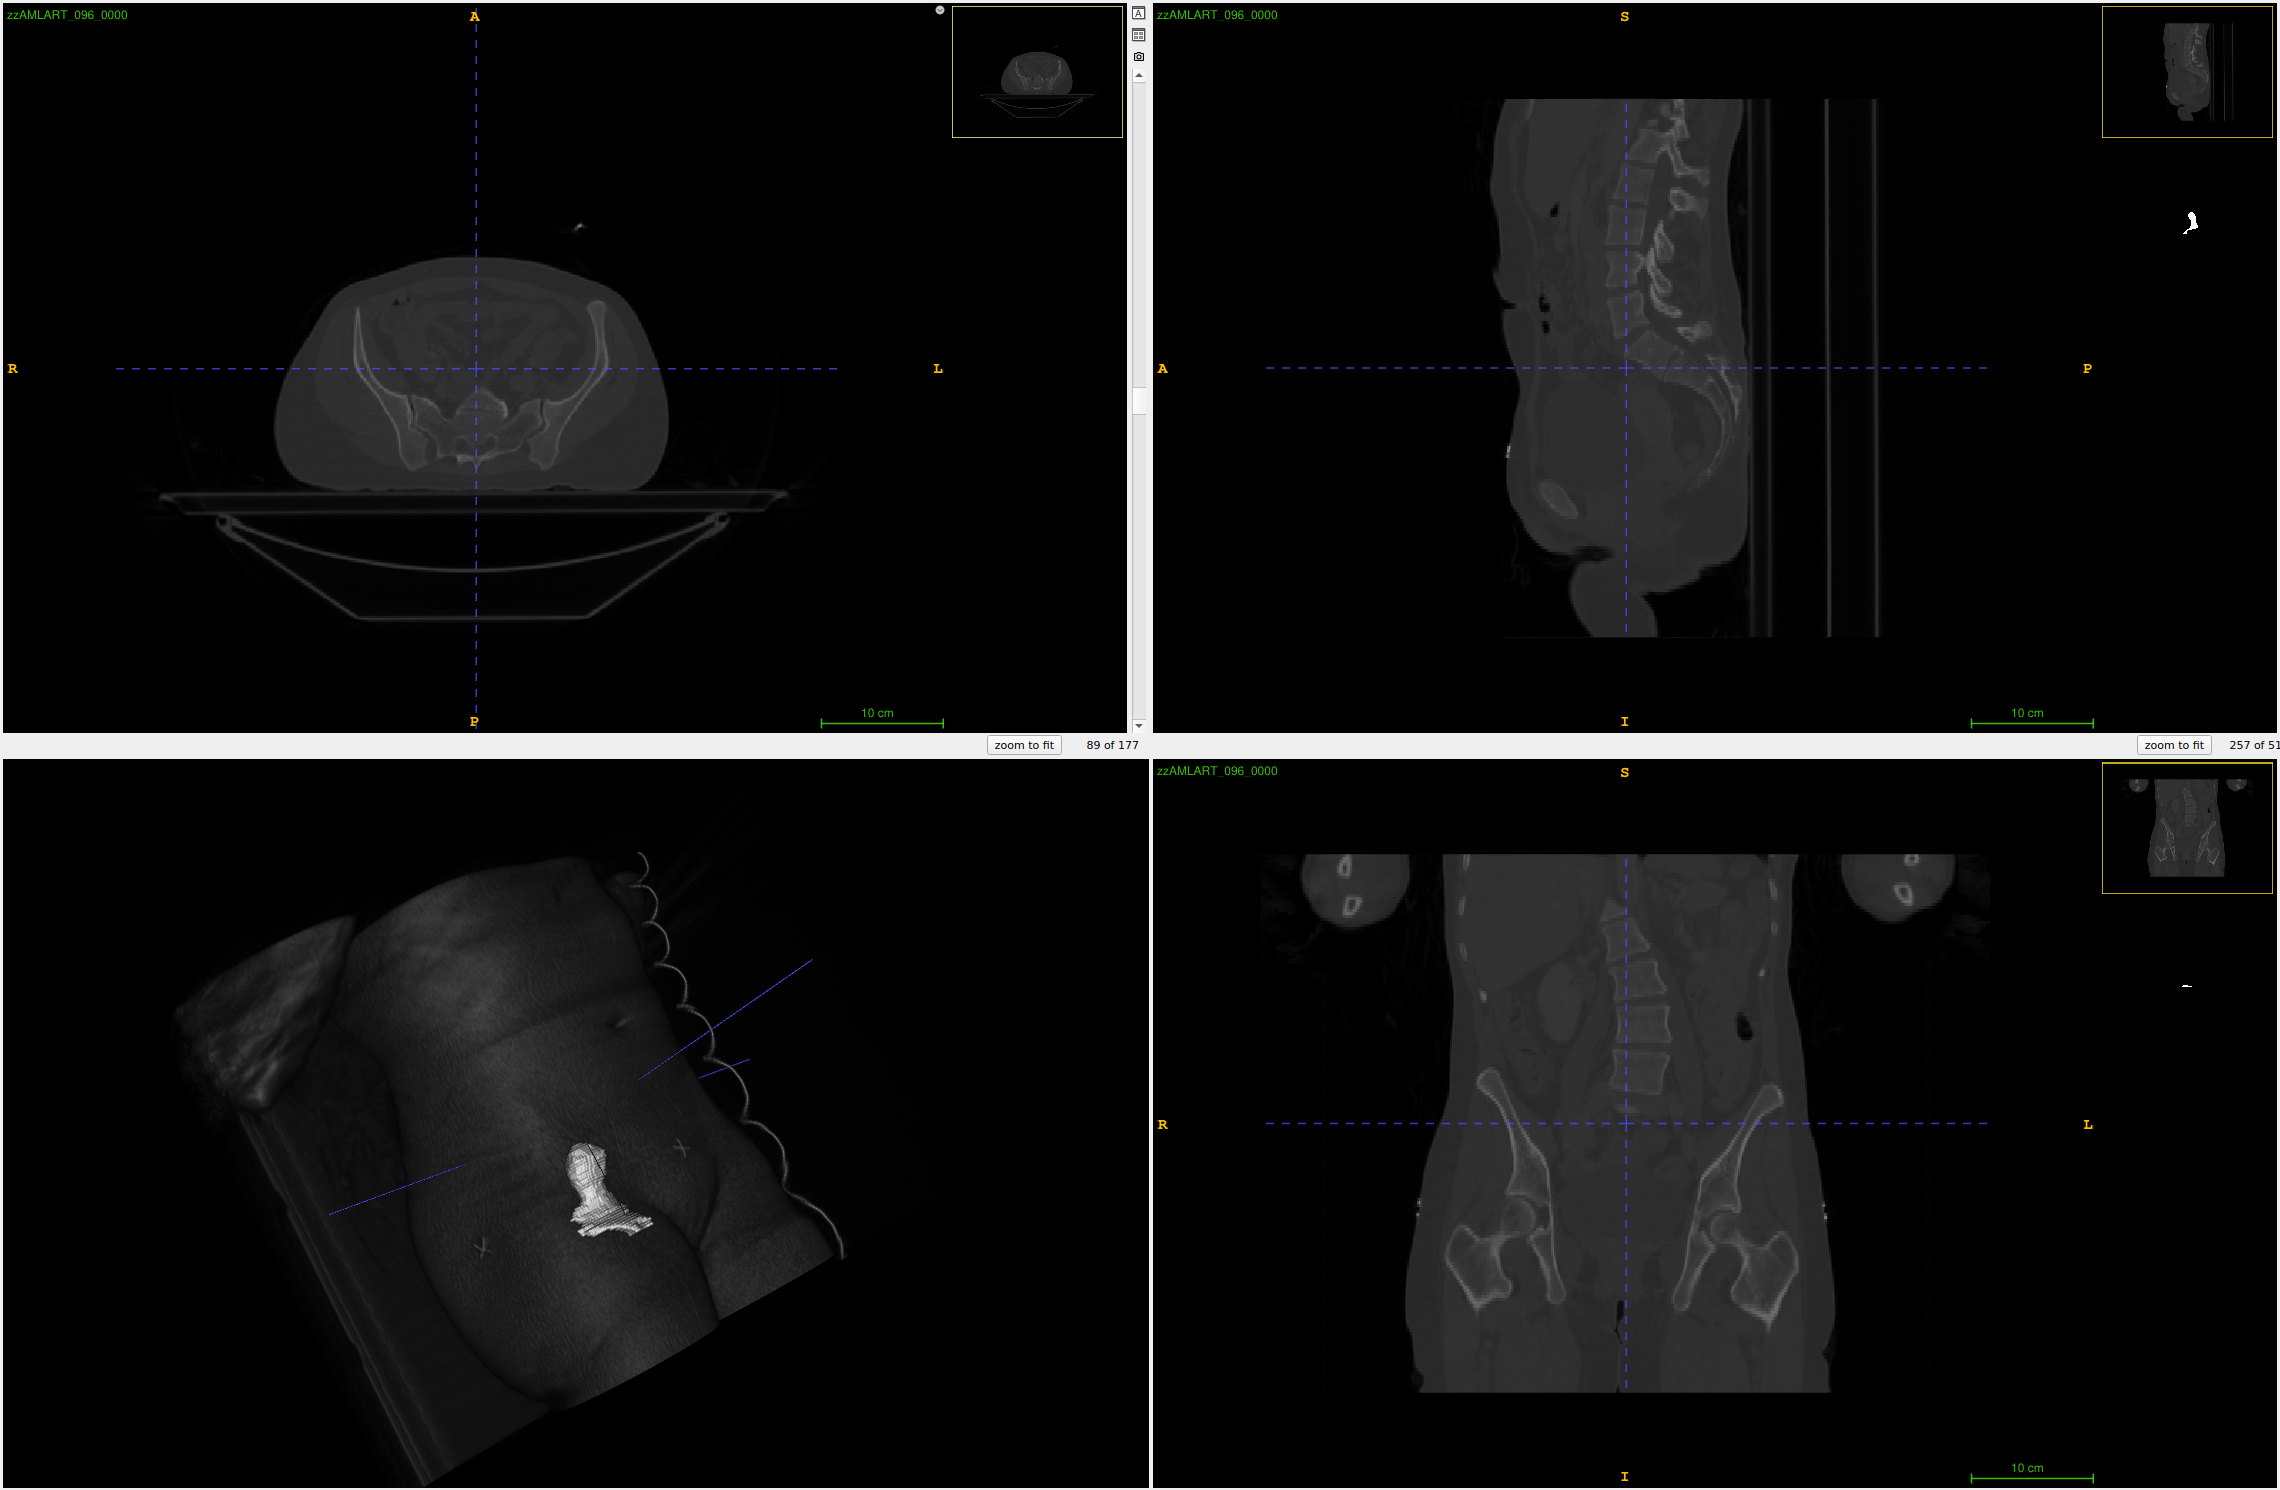
\includegraphics[width=0.6\textwidth]{images/CTVp.png}
    \caption{ItkSnap view of the CTVp}\label{fig:CTVn}
\end{figure}

\textbf{CTVp} stands for Primary Clinical Target Volume. Clinical Target volume covering area where there may be local microscopic spread (uterus, cervix, upper vagina, primary tumour)~\cite{AMLART-data}. This is the area that contains the tumour.

It is made from the following structures:

\begin{itemize}
    \item GTVp - Primary gross tumour volume (Visible Primary Tumour)
    \item Whole cervix (this will contain at least most of the GTVp. The GTVp could however grow out of this structure)
    \item Uterus - (contains the whole cervix)
    \item Vagina for CTV - (2cm below the lowest slice containing the cervix or GTVp). The whole vagina is initially contoured, then the vagina for CTV is made by copying the whole vagina and deleting unnecessary slices. 
\end{itemize}

We have that $Whole\ Cervix + GTVp = High\ Risk\ CTV$ which clinitians advise may be easier to train on since the GTVp will be harder to learn due to large variation in samples.

We also have that $High\ risk\ CTV + Uterus + vagina\ for\ CTV = CTVp$

\subsubsection{CTVn}

\begin{figure}[H]
    \centering
    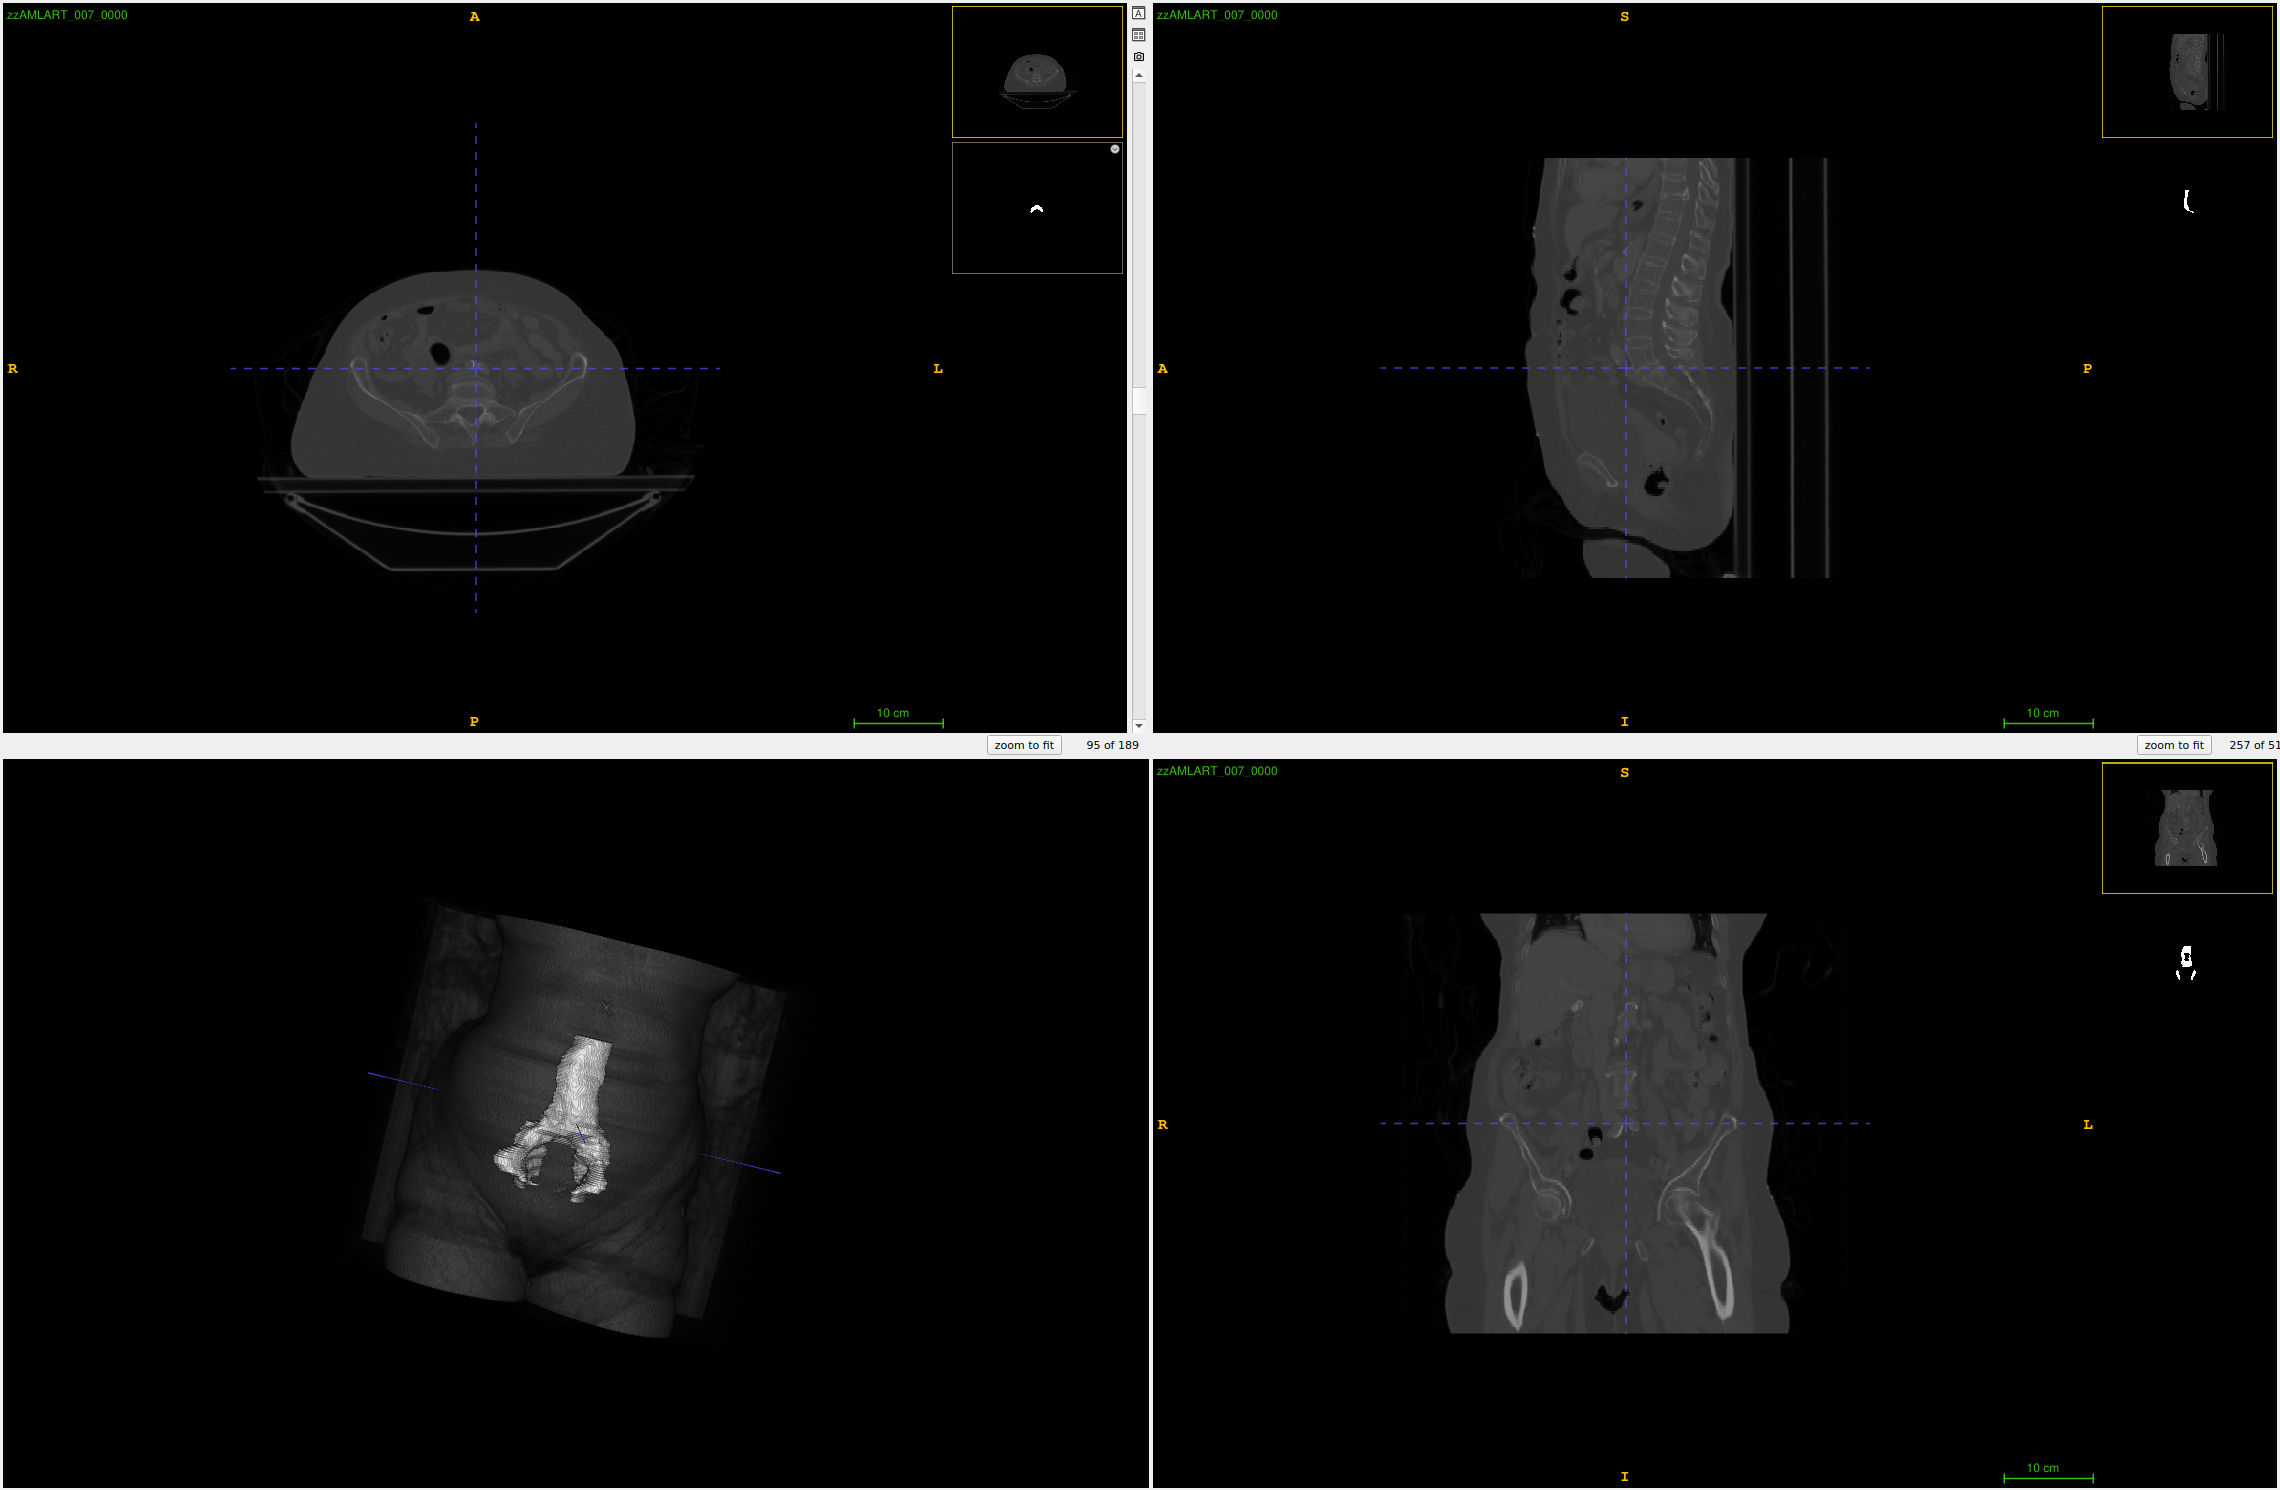
\includegraphics[width=0.6\textwidth]{images/CTVn.png}
    \caption{ItkSnap view of the CTVn}\label{fig:CTVn}
\end{figure}

\textbf{CTVn} stands for Nodal Clinical Target Volume. Clinical Target volume covering area where there may be microscopic spread to lymph nodes. Drawn based on set margins around pelvic blood vessels. Includes pelvic lymph nodes, common iliac lymph nodes and para-aortic lymph nodes~\cite{AMLART-data}.

There are three groups of lymph nodes. In clinical practice, the number of these groups included in the CTV varies in each patient, depending on how advanced the disease is. Pathological lymph nodes (GTVn) are also included

\begin{itemize}
    \item Pelvic lymph nodes
    \item Common iliac lymph nodes
    \item Para-aortics
    \item GTVn (Gross Nodal Tumour) (usually included within the CTV nodes)
\end{itemize}

We have that $GTVn + Common\ iliac + pelvic + para-aortics = Nodal\ CTV$

\subsubsection{Parametrium}

\begin{figure}[H]
    \centering
    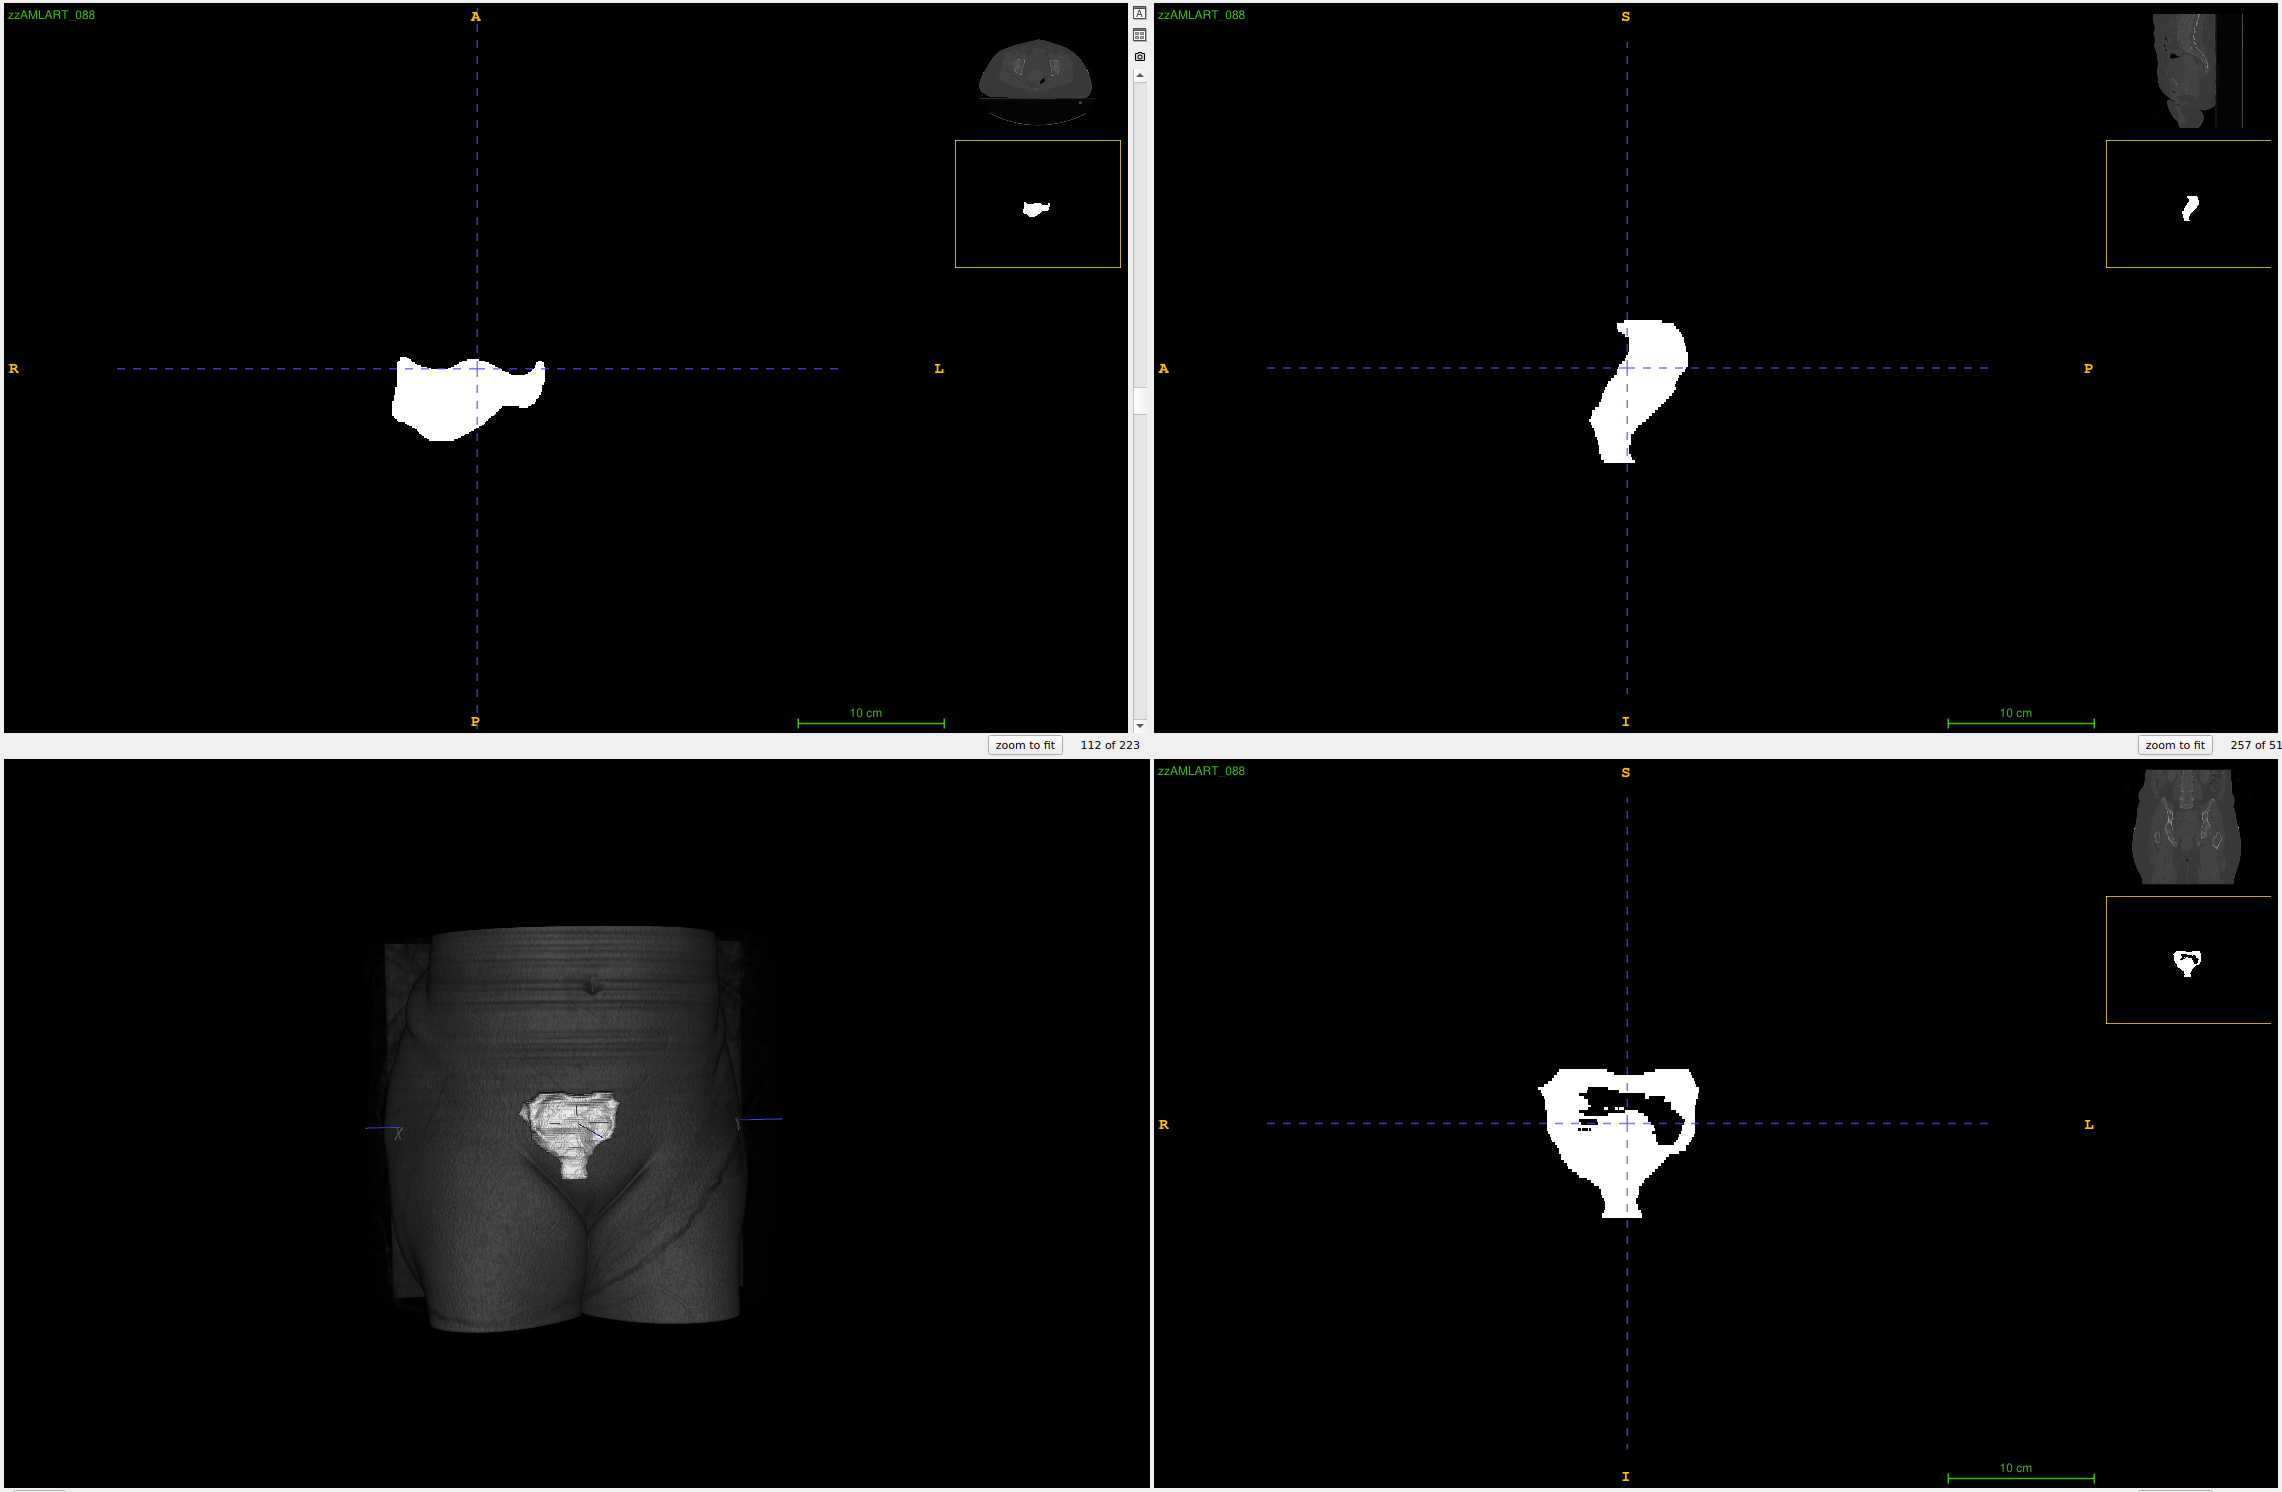
\includegraphics[width=0.6\textwidth]{images/Parametrium.png}
    \caption{ItkSnap view of the Parametrium}\label{fig:CTVn}
\end{figure}

\textbf{Parametrium/ Paravagina} is the tissue surrounding the cervix/vagina - at risk of local spread. Drawn as a complete structure, then also to the level of the vagina included in the CTVp~\cite{AMLART-data}.

Parametrium and Paravagina (whole and for CTV)  Contour whole Parametrium and Paravagina. Parametrium and Paravagina for CTV can be made by copying the whole paravagina and editing back to the level of vagina to be included

\printbibliography %Prints bibliography

\end{document}